\section{Procesos aleatorios estacionarios}\label{sec.estoc}

\begin{figure}[h]
    \centering\begin{minipage}{\textwidth}
    \bpgf{Imagenes/estoc/estoc-1}
    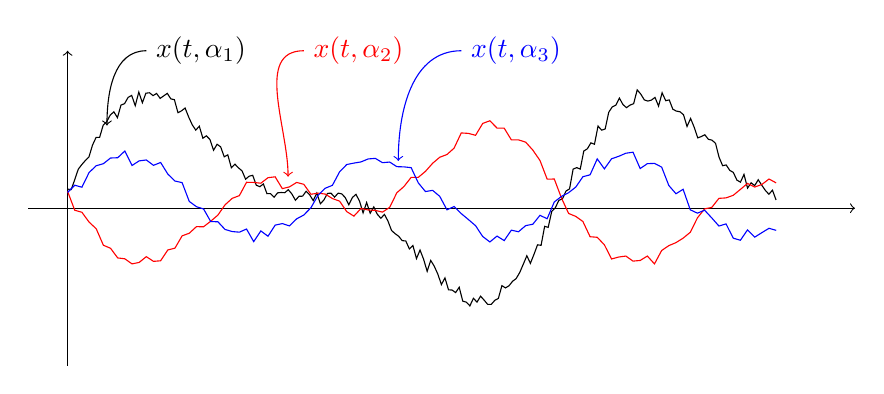
\begin{tikzpicture}
        \draw [->] (-0.5,0) -- (10,0);
        \draw [->] (0,-2) -- (0,2);
        \draw [samples=200,domain=0:9] plot (\x,{0.15+sin(\x r)*(1+cos(\x r +1))+0.1*rand});
        \draw [->] (1,2) node [anchor=west] {$x(t,\alpha_1)$} to [out=180,in = 90] (0.5,1.05);
        \draw [samples=100,domain=0:9,color=red] plot (\x, {0.15-sin(\x r)*(0.5+cos(\x r +1))+0.1*rand});
        \draw [->,color=red] (3,2) node [anchor=west,color=red] {$x(t,\alpha_2)$} to [out=180,in=90] (2.8,0.4);
        \draw [samples=100,domain=0:9,color=blue] plot (\x, {0.15+sin(\x r)*(cos(\x r +1))+0.1*rand});
        \draw [->,color=blue] (5,2) node [anchor=west,color=blue] {$x(t,\alpha_3)$} to [out=180,in=90] (4.2,0.6);
    \end{tikzpicture}
    \endpgfgraphicnamed\end{minipage}
    \end{figure}

Sorteo una señal a través de $\alpha\in\Omega$, espacio de probabilidad.
\begin{itemize}
    \item Para cada sorteo $\alpha$ tengo una {\em trayectoria}
    $X(t,\alpha)$.
    \item Para cada $t$ tengo una variable aleatoria $X(t)$. En particular, tiene una distribución de probabilidad $F_{X(t)}(x)$ y puedo calcular
    momentos $E\left[X(t)\right]$, $E\left[X^2(t)\right]$: promedios en el ``ensemble'', para $t$ fijo.
\end{itemize}

La familia de distribuciones \emph{conjuntas} de las variables
aleatorias $X(t_1),\ldots,X(t_n)$ para cualesquiera tiempos
$(t_1,t_2,\ldots,t_n)$ caracteriza al proceso.

En general la distribuci\'on del proceso puede variar en el
tiempo. Un proceso se dice {\bf estrictamente estacionario} si
esto no ocurre, es decir que la distribución de
$\left(X(t_1),\ldots,X(t_n)\right)$ es igual a la de
$\left(X(t_1+\tau),\ldots,X(t_n+\tau)\right)$ para cualquier
$\tau$.

Se trabaja en general una noción más amplia de proceso
estacionario, a definirse a continuación. Notamos que cualquier
proceso estrictamente estacionario con momento de segundo orden
finito cumple también la definición que sigue.

\subsection*{Proceso estacionario (sentido amplio)}
Un proceso aleatorio $X(t)$ es estacionario en sentido amplio si
se cumple:
\begin{enumerate}
    \item $E\left[X(t)\right]=\mu$, constante en el tiempo.
    \item $E\left[X(t)X(t-\tau)\right]=R_X(\tau)$ (autocorrelación en sentido aleatorio) independiente de $t$.
\end{enumerate}

\newpage

{\bf Ejemplo 1: Sinusoide de fase aleatoria.}

%\begin{ejemplo}[Sinusoide de fase aleatoria]$\phantom{1}$

$X(t)=\cos(\omega_0t+\theta)$, con $\theta$ variable aleatoria de
distribución uniforme en $[0,2\pi]$. Esto modela una señal
sinusoidal con frecuencia conocida pero de la que no tenemos
información de sincronismo.

\begin{align*}
    E\left[X(t)X(t-\tau)\right]     & = E\left[\cos(\omega_0t+\theta)\cos\left(\omega_0(t-\tau)+\theta\right)\right]\\
                    & = E\left[\frac{\cos(\omega_0\tau)}{2}+\frac{\cos(2\omega_0t-\omega_0\tau+2\theta)}{2}\right]\\
                    & = \frac{1}{2}\cos(\omega_0\tau)+\frac{1}{2\pi}\int_0^{2\pi}\frac{\cos(2\omega_0t-\omega_0\tau+2\theta)}{2}\d\theta\\
                    & = \frac{1}{2}\cos(\omega_0\tau).
\end{align*}
Por lo tanto $R_X(\tau)=\frac{1}{2}\cos(\omega_0\tau)$. Por un
cálculo similar tenemos que $E\left[X(t)\right]=0$, y por lo tanto
el proceso es estacionario en sentido amplio.
%\end{ejemplo}

%\begin{ejemplo}[Onda binaria aleatoria] $\phantom{1}$

{\bf Ejemplo 2: Onda binaria aleatoria} \\

    \begin{minipage}{0.65\textwidth}
        \resizebox{\textwidth}{!}{
        \bpgf{Imagenes/estoc/estoc-2}
        \begin{tikzpicture}
            \draw [->] (-0.5,0) -- (7,0);
            \draw [->] (0,-1.5) -- (0,1.5);
            \path (0,1) node [anchor=east] {$1$} -- (0,-1) node [anchor=east] {$-1$};
            \draw (0,1) -- (1,1) -- (1,-1) -- (3,-1) -- (3,1) -- (4,1) -- (4,-1) -- (5,-1) -- (5,1) -- (6.5,1);
            \path (1,0) node [anchor=north west] {$T$};
            \draw [dotted,thin] (2,0) node [anchor=south] {$2T$} -- (2,-1);
        \end{tikzpicture}
        \endpgfgraphicnamed
        }
    \end{minipage}
    \hfill
    \begin{minipage}{0.3\textwidth}
        $X(t)=X_k$ constante en $[kT,(k+1)T)$;

        $\lbrace X_k\rbrace$ sucesión de V.A. independientes,
        distribuidas en $\pm 1$ con probabilidad $\frac{1}{2}$.
    \end{minipage}

    \noindent Es facil ver que $E\left[X(t)\right]=0$. ¿$X(t)$ es estacionario? No, los instantes $\lbrace kT\rbrace$ son ``especiales''. En
    particular, $E\left[X(t)X(t-\tau)\right]$ va a depender no
    sólo de $\tau$, sino también de si hay o no una frontera de
    intervalo $kT$ entre estos tiempos. Por ejemplo:
    \begin{gather*}
        X\left(\tfrac{T}{4}\right)=X\left(\tfrac{3T}{4}\right)\ \ \text{con probabilidad $1$, pero
        } \
        P\left(X\left(\tfrac{3T}{4}\right)=X\left(\tfrac{5T}{4}\right)\right)=\frac{1}{2},
    \end{gather*}
de donde se deduce que $E\left[X(t)X(t-\frac{T}{2})\right]$ vale
$1$ para $t=\frac{3}{4}$, y vale $0$ para
    $t=\frac{5}{4}$. O sea que no tenemos una autcorrelación
    dependiente solo de $\tau$.

    Una forma de definir una onda binaria aleatoria estacionaria es agregar un retardo aleatorio
    $D$, uniforme en $[0,T]$, e independiente de $X(t)$.
    Intuitivamente, esto quita el sincronismo de los instantes
    $kT$ y ``todos los tiempos se vuelven iguales".

    Formalmente, sea $Y(t)=X(t-D)$. Este proceso es constante,
    igual a $X_k$ en el intervalo $[kT+D,(k+1)T+D)$.
Fijados dos tiempos, $t-\tau$, $t$ sea ``$A$" el
    suceso ``ambos tiempos caen en el mismo intervalo (mismo
    $k$)". Como la distribución de $D$ es uniforme en $[0,T]$, la probabilidad de
    $A$ decrece linealmente con $\tau$ hasta $\tau = T$, donde
    se vuelve nula. Es decir
    \[P(A) = \begin{cases}
                1-\frac{|\tau|}{T} & 0\leq |\tau|\leq T,\\
                0 & |\tau|>T.
            \end{cases}\]
Calculamos $E[Y(t)Y(t-\tau)]$, utilizando la probabilidad
condicional a los sucesos $A$ y su complemento $A^c$. Si ocurre
$A$, $Y(t)=Y(t-\tau)=\pm 1$ por tanto el valor esperado
condicional es  $E[Y(t)Y(t-\tau)|A]= 1$. Si en cambio ocurre
$A^c$, $Y(t)$, $ Y(t-\tau)$ son independientes y el valor esperado
es cero. Combinandolos
\begin{align*}
E[Y(t)Y(t-\tau)] & = E[Y(t)Y(t-\tau)|A] \cdot P(A) +
E[Y(t)Y(t-\tau)|A^c]\cdot P(A^c) \\
& = 1\cdot P(A)+0\cdot P(A^c)\\
&= P(A).
\end{align*}
Como $P(A)$ depende sólo de $\tau$, $Y(t)$ es estacionario con
autocorrelación \[ R_Y(\tau)=\begin{cases}
                1-\frac{|\tau|}{T} & 0\leq |\tau|\leq T,\\
                0 & |\tau|>T.
            \end{cases}\]

\subsection*{Relación entre correlaciones temporales y probabilísticas}

Para un proceso estacionario tenemos entonces dos definiciones de
autocorrelación:
\begin{itemize}
    \item La aleatoria $R_X(\tau)=E[X(t)X(t-\tau)]$.
    \item En cada trayectoria $x(t)= X(t,\alpha)$ (cada resultado del sorteo), podemos calcular la autocorrelación determinística
    $r_x(\tau) = \lim_{T\rightarrow\infty} \frac{1}{T}\int^{\frac{T}{2}}_{-\frac{T}{2}}
    x(t)x(t-\tau)\d t.$
\end{itemize}
En principio, la segunda podría depender de $\alpha$ (el sorteo),
y no tendría por qué coincidir con la primera. Sin embargo, en una
clase importante de procesos, llamados \emph{ergódicos}, se
verifica la igualdad de las medias temporales y probabilísticas.
%
%%\paragraph{Preguntas:}
%\begin{itemize}
%    \item ¿La segunda depende de?
%    \item ¿Son iguales?
%\end{itemize}
%
%Este concepto, iguadad de medias temporales y probabilísticas se
%llama  del proceso.

\paragraph{Recordar:} ``Ley de los grandes números'' en probabilidad.

Dado $X_1,X_2,\ldots,X_k,\ldots$ sucesión de V.A. independientes,
idénticamente distribuidas (I.I.D.), con $E[X_k]=\mu$. Entonces
con probabilidad $1$,
\[\frac{X_1+X_2+\cdots+X_k}{k}\xrightarrow[k\rightarrow\infty]{}\mu.\]

Promedio temporal $=$ promedio probabilístico.

Esto es un ejemplo de \emph{ergodicidad} (en la media). Vale para
variables independientes, o en aquellas en que la dependencia se
``apaga'' al alejarnos en el tiempo.

\paragraph{Versión de tiempo continuo:} $X(t)$  ergódico en el media si
\[\lim_{T\rightarrow\infty}\frac{1}{T}\int^{\frac{T}{2}}_{-\frac{T}{2}}X(t)\d t \underset{\text{con prob $1$}}{=}E\left[X(t)\right].\]

$X(t)$ ergódico en el autocorrelación si:
\[\lim_{T\rightarrow\infty}\frac{1}{T}\int^{\frac{T}{2}}_{-\frac{T}{2}}X(t)X(t-\tau)\d t \underset{\text{con prob $1$}}{=}E\left[X(t)X(t-\tau)\right].\]
En otras palabras $R_X(\tau)=r_X(\tau)$ con probabilidad 1.

Intuitivamente, en un proceso ergódico la trayectoria de
$X(t,\alpha)$ toma a lo largo del tiempo valores representativos
de la distribución, de modo que los promedios temporales
reconstruyen el promedio en todos los posibles sorteos.

En adelante, supondremos que todos los procesos estacionarios que
encontraremos son ergódicos. Los promedios en el tiempo y en la
muestra coinciden.

\subsection*{Densidad espectral de potencia de un proceso ergódico}

Si se cumple la identidad $R_X(\tau)=r_X(\tau)$, podemos utilizar
la transformada de Fourier de la primera para calcular la densidad
espectral de potencia de las trayectorias del proceso. Lo hacemos
en los ejemplos anteriores:


\begin{enumerate}
    \item Sinusoide de fase aleatoria, $\cos(\omega_0t+\theta)$.
    \[R_X(\tau)=\frac{1}{2}\cos(\omega_0\tau)\Rightarrow S_X(f)=\frac{\delta(f+f_0)+\delta(f-f_0)}{4}.\]

    \paragraph{Nota: } el mismo resultado se obtiene para sinusoides determinísticas sin fase aleatoria. Esto no sorprende, ya que el cambio de fase no afecta la autocorrelación.

    \item Onda binaria aleatoria con retardo uniforme
    \[R_Y(\tau)=1-\frac{|\tau|}{T} \ \ \mbox{ para } |\tau|\leq T \quad \Rightarrow S_Y(f) = T\left[\sinc^2(\pi f T)\right].\]
    Esto nos dice donde se distribuye la potencia de una onda
    digital, lo cual sería difícil de obtener sin recurrir a la
    ergodicidad.
    \paragraph{Nota: } sin  el retardo aleatorio el proceso deja de ser estacionario, no puedo hallar $R_X(\tau)$.
    Pero en cada trayectoria, el retardo no afecta $r_x$, por lo tanto se puede argumentar que la densidad espectral de
    potencia calculada vale para la onda binaria sin retardo.
    \end{enumerate}

\subsection*{Procesos Gaussianos}

Un proceso es Gaussiano si las distribuciones conjuntas de
$\left(X(t_1),\ldots,X(t_n)\right)$ son normales (multivariadas)
para cualesquiera $t_1,\ldots,t_n$.  En particular, para cada $t$
$X(t)$ es una variable aleatoria normal, de densidad
$f_X(x)=\frac{1}{\sqrt{2\pi}\sigma}\e^{-\frac{(x-\mu)^2}{2\sigma^2}}$.

\noindent {\bf Propiedad:} una operación lineal (en particular,
filtrado) aplicada a un proceso Gaussiano da un resultado
Gaussiano.



\noindent {\bf Ejemplo:}
    \begin{figure}[htb]
        \centering\begin{minipage}{\textwidth}
        \bpgf{Imagenes/estoc/estoc-3}
        \begin{blockdiagram}
            \matrix[row sep=5mm, column sep=10mm]{
                \node[etiqueta] (inicio) {\begin{minipage}{5cm}
                                            Ruido blanco, Gaussiano, media $0$, densidad espectral de potencia $\frac{\eta}{2}$
                                          \end{minipage}}; & \node [block] (filtro) {PASABAJOS $B$}; & \node[etiqueta] (final) {\quad $n(t)$};\\
            };
            \draw[->] (inicio) -- (filtro);
            \draw[->] (filtro) -- (final);
        \end{blockdiagram}
        \endpgfgraphicnamed\end{minipage}
    \end{figure}
    \FloatBarrier
\paragraph{Pregunta} ¿Cuál es la probabilidad de que $n(t)>K$?

Primero, observamos que  $n(t)$ es un proceso estacionario de
densidad espectral de potencia
$S_n(f)=\frac{\eta}{2}\left|\hat{H}(f)\right|^2$, donde
$\hat{H}(f)$ es la transferencia del pasabajos.  Suponemos que es
ergódico. También es Gaussiano. Por lo tanto $n(t)$ tiene
distribución normal, con parámetros
\begin{align*}
    \mu&=0,\\
    %\begin{aligned}
        \sigma^2    & = E\left[x^2(t)\right]\\
                & = R_X(0)\\
                & = \frac{\eta}{2}\int_{-\infty}^\infty
                \left|\hat{H}(f)\right|^2\d f \\
                & = \eta B.
    \end{align*}
%\end{gather*}
Esto permite calcular la probabilidad deseada:
\begin{align*}
P\left(n(t)>K\right) & = %\int_K^\infty f_n(x)\d x =
\frac{1}{\sqrt{2\pi}\sigma}\int_K^\infty
\e^{-\frac{x^2}{2\sigma^2}}\d x =
\frac{1}{\sqrt{2\pi}}\int_{\frac{K}{\sigma}}^\infty
\e^{-\frac{z^2}{2}}\d z = Q\left(\frac{K}{\sigma}\right)=
Q\left(\frac{K}{\sqrt{\eta B}}\right),
\end{align*}
donde \[ Q(x) = 1 - F_X(x) \] es la ``cola" de la distribución
normal $(0,1)$. Volveremos a esto en más detalle al estudiar
detección digital.
